\documentclass[urlcolor=blue,dvipsnames]{beamer}

\usepackage[utf8]{inputenc}
\usepackage{fancybox,fancyvrb}
\usepackage{environ,xspace}
\usepackage{tikz}
\hypersetup{colorlinks,linkcolor=,urlcolor=cyan}

\beamertemplatenavigationsymbolsempty
\setbeamertemplate{footline}[frame number]
\usetheme{Pittsburgh}

\newcommand\enumnum[1]{{\renewcommand{\insertenumlabel}{#1}%
      \usebeamertemplate{enumerate item} \,}}

\newcommand{\grad}{\nabla}
\newcommand{\ih}{\boldsymbol{\hat{\textbf{\i}}}}
\newcommand{\jh}{\boldsymbol{\hat{\textbf{\j}}}}
\newcommand{\vF}{\boldsymbol{\vec{\textbf{F}}}}
\newcommand{\Matlab}{\textsc{Matlab}\xspace}
\newcommand{\Octave}{\textsc{Octave}\xspace}


\title{6.1 Power series solutions of DEs \\ (and review)}

\subtitle{a lesson for MATH F302 Differential Equations}

\author{Ed Bueler, Dept.~of Mathematics and Statistics, UAF}

\date{\tiny \today}


\begin{document}
\setbeamertemplate{itemize item}{$\bullet$}
\setbeamertemplate{itemize subitem}{$\circ$}


\begin{frame}
\titlepage

\centerline{\tiny for textbook: \, D. Zill, \emph{A First Course in Differential Equations with Modeling Applications}, 11th ed.}
%\color{green!40!blue}
\end{frame}


\begin{frame}{we already use power series}

\begin{itemize}
\item the exponential function is \emph{defined} by an infinite series:
    $$e^x = 1 + x + \frac{x^2}{2} + \frac{x^3}{3!} + \dots$$
    \begin{itemize}
    \item there are other ways to define it but series is the default def.
    \item see \href{https://en.wikipedia.org/wiki/Characterizations_of_the_exponential_function}{``characterizations of the exponential function''} at wikipedia
    \end{itemize}
\item a \emph{power series} is an infinite sum of coefficients times powers of $x$; the above is a power series
\item \emph{exercise.} from the above series for $y(x)=e^x$, show
    $$y'=y \,\, \text{ and } \,\, y(0)=1$$
\end{itemize}

\vspace{30mm}
\end{frame}


\begin{frame}{a series with unknown coefficients}

\noindent \emph{exercise.}  find the coefficients in the power series
    $$y(x) = c_0 + c_1 x + c_2 x^2 + c_3 x^3 + c_4 x^4 + \dots$$
so that $y(x)$ solves the IVP: \hfill $y'+3y=0, \, y(0) = 7$

\vspace{60mm}
\end{frame}


\begin{frame}{series solutions of DEs: the basic idea}

\begin{itemize}
\item the last slide, and the next slide, show the basic idea:

\medskip
\begin{quotation}
\noindent \alert{substitute a series with unknown coefficients into the DE, and thereby find the coefficients}
\end{quotation}

\item with appropriate initial conditions one can get \emph{one} series solution
\item without initial conditions one gets a family of series solutions, i.e.~the general solution
\end{itemize}
\end{frame}


\begin{frame}{exercise \#37 in \S 6.1}

\noindent \emph{exercise.}  find the general solution by using a power series with unknown coefficients:
    $$y'=xy$$

\vspace{70mm}
\end{frame}


\begin{frame}{review of series}

\begin{itemize}
\item you already have the main idea
\item reviewing only needed to be faster/clearer/smarter
\item must recall knowledge from calculus II:

    \begin{enumerate}
    \item some familiar series
        \begin{itemize}
        \item including little tricks for fiddling with familiar series to get other series
        \end{itemize}
    \item how summation notation works
        \begin{itemize}
        \item including shifting the index of summation
        \end{itemize}
    \item what are the \emph{radius of convergence} and the \emph{interval of convergence}, and how to find them
    \end{enumerate}

\bigskip
\item I'll do some reviewing in these slides, but \dots
\item to do \emph{your} review, start by \alert{reading the text in section 6.1}!!
\end{itemize}
\end{frame}


\begin{frame}{exponential and related series}

\begin{itemize}
\item we know that for any $x$,

\vspace{-2mm}
    $$e^x = 1 + x + \frac{x^2}{2} + \frac{x^3}{3!} + \frac{x^4}{4!} + \dots = \sum_{k=0}^\infty \frac{x^k}{k!}$$

\vspace{-3mm}
    \begin{itemize}
    \item $0!=1$ and $1!=1$ by definition
    \item factorial $n!$ grows faster than $b^n$ for any $b$ \dots why? so what?
    \end{itemize}
\item split even and odd terms:
\begin{align*}
\cosh x &= \hspace{80mm} \\
\sinh x &=
\end{align*}

\vspace{-3mm}
    \begin{itemize}
    \item $\displaystyle \cosh x = \frac{e^x+e^{-x}}{2}$, \, $\displaystyle \sinh x = \frac{e^x-e^{-x}}{2}$
    \end{itemize}
\item use $e^{i\theta} = \cos\theta + i \sin\theta$:
\begin{align*}
\cos x &= \hspace{80mm} \\
\sin x &=
\end{align*}
    
\end{itemize}
\end{frame}


\begin{frame}{geometric series}

\begin{itemize}
\item recall:
    $$\frac{1}{1-x} = 1 + x + x^2 + x^3 + x^4 + \dots = \sum_{n=0}^\infty x^n$$

\vspace{-3mm}
    \begin{itemize}
    \item why?

\vspace{20mm}
    \item for which $x$?
    \end{itemize}

\vspace{20mm}
\end{itemize}
\end{frame}


\begin{frame}{related to geometric series}

\begin{itemize}
\item geometric series for $x\in(-1,1)$:
    $$\frac{1}{1-x} = 1 + x + x^2 + x^3 + x^4 + \dots = \sum_{n=0}^\infty x^n$$
\item substitution gives other series:
   $$\frac{1}{1+x^2} = \hspace{80mm}$$

\bigskip
\item integration gives other series:
   $$\ln(1+x) = \hspace{80mm}$$

   $$\arctan(x) = \hspace{80mm}$$

\bigskip
\end{itemize}
\end{frame}


\begin{frame}{familiar series worth knowing}

\begin{itemize}
\item somewhat by accident I've explained all of these 8 series:
\end{itemize}

\bigskip
\hfill 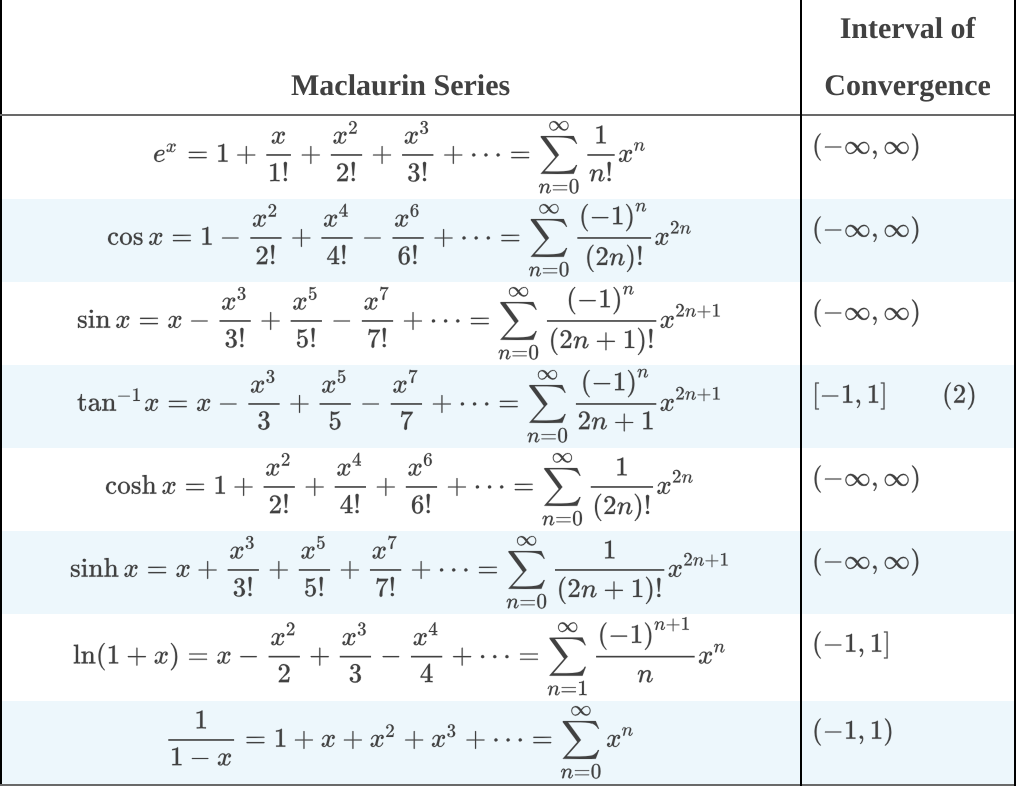
\includegraphics[width=0.7\textwidth]{figs/familiarseries}
\end{frame}


\begin{frame}{exercise \#14 in \S 6.1}

\noindent \emph{exercise.}  Use a familiar series to find the Maclaurin series of the given function.  Write your answer in summation notation.

$$f(x)=\frac{x}{1+x^2}$$

\vspace{50mm}
\end{frame}


\begin{frame}{base point}

\begin{itemize}
\item a general power series is
    $$\sum_{n=0}^\infty c_n (x-a)^n = c_0 + c_1 (x-a) + c_2 (x-a)^2 + \dots$$
    \begin{itemize}
    \item $a$ is the \emph{base point}; the series is \emph{centered at $a$}
    \item note that $f(a)=c_0$
    \end{itemize}
\item \emph{exercise.}  find a power series centered at $a=5$:
    $$f(x) = \sin(2x) \hspace{80mm}$$

\vspace{30mm}
\end{itemize}
\end{frame}


\begin{frame}{convergence of power series}

\begin{itemize}
\item \emph{fact.} for the series
there is a value $0 \le R \le \infty$ where the series converges if $a-R < x < a+R$ and it diverges if $x<a-R$ or $x>a+R$
    \begin{itemize}
    \item equivalently ``$|x-a|<R$''
    
     and ``$|x-a|>R$'' resp.
    \end{itemize}

\vspace{-10mm}

\hfill 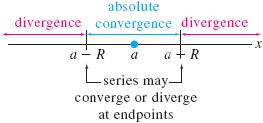
\includegraphics[width=0.4\textwidth]{figs/convergediverge}

\vspace{-10mm}
\item \emph{exercise.} substitute $x=\pm1$ into
   $$\ln(1+x) = \sum_{n=1}^\infty \frac{(-1)^{n+1}}{n} x^n \hspace{50mm}$$
do the resulting series converge?

\vspace{25mm}
\end{itemize}
\end{frame}


\begin{frame}{exercise \#31 in \S 6.1}

\noindent \emph{exercise.}  Verify by substitution that the given power series is a solution; use summation notation.  Radius of convergence?

$$y=\sum_{n=0}^\infty \frac{(-1)^n}{n!} x^{2n}, \qquad\quad y'+2xy=0$$

\vspace{50mm}
\end{frame}


\begin{frame}{exercise \#31, cont.}

\end{frame}


\begin{frame}{exercise \#5 in \S 6.1}

\noindent \emph{exercise.}  Find the interval and radius of convergence:
    $$\sum_{k=1}^\infty \frac{(-1)^k}{10^k} (x-5)^k$$

\begin{itemize}
\item using ratio test:

\vspace{20mm}
\item using geometric series:

\vspace{20mm}
\end{itemize}
\end{frame}


\begin{frame}{expectations}

\begin{itemize}
\item just watching this video is \emph{not} enough!
     \begin{itemize}
     \item see ``found online'' videos at

     \centerline{\href{https://bueler.github.io/math302/week9.html}{\tt \color{cyan} bueler.github.io/math302/week9.html}}
     \item \emph{read} section 6.1 and 6.2 in the textbook
     \item \emph{do} the WebAssign exercises for section 6.1
     \end{itemize}
\end{itemize}
\end{frame}

\end{document}

